\documentclass[11pt,a4paper]{article}

% ---------------------------------------------------------------------------
% Packages
% ---------------------------------------------------------------------------
\usepackage[margin=2.2cm]{geometry}
\usepackage[T1]{fontenc}
\usepackage{lmodern}
\usepackage{booktabs}
\usepackage{tabularx}
\usepackage{array}
\usepackage{xcolor}
\usepackage{listings}
\usepackage{float}
\usepackage{caption}
\usepackage{enumitem}
\usepackage{tikz}
\usetikzlibrary{positioning,arrows.meta,shapes.geometric,fit,calc}
\usepackage[hidelinks]{hyperref}

\definecolor{codebg}{RGB}{246,246,246}
\definecolor{codeframe}{RGB}{200,200,200}
\definecolor{okgreen}{RGB}{0,128,60}
\definecolor{errred}{RGB}{180,30,30}
\definecolor{warnorange}{RGB}{200,110,0}

\lstset{
  basicstyle=\ttfamily\footnotesize,
  backgroundcolor=\color{codebg},
  frame=single,
  rulecolor=\color{codeframe},
  breaklines=true,
  columns=fullflexible,
  keepspaces=true,
  showstringspaces=false,
  xleftmargin=4pt,
  xrightmargin=4pt
}

% protocol symbols and file names contain underscores
\newcommand{\sym}[1]{\texttt{\detokenize{#1}}}
\newcommand{\yes}{\textcolor{okgreen}{\textbf{yes}}}
\newcommand{\no}{\textcolor{errred}{\textbf{no}}}

\title{\textbf{Thrust 1: Implementation-Grounded Specification Model}\\
\textbf{First Results on 5G NAS}}
\author{%
  Technical Report --- Ajoy Dey\\
  \small B.Sc.\ CSE, BUET \;$|$\; \texttt{ajoydey00001@gmail.com} \;$|$\; \texttt{ajoydey00001.github.io}\\
  \small Prepared for Dr.\ Imtiaz Karim, SysNetS Lab, The University of Texas at Dallas}
\date{\small 14 October 2026 \;---\; version 2 (budget-limited srsUE hypothesis)}

\begin{document}
\maketitle

% ---------------------------------------------------------------------------
\begin{abstract}
Differential testing of cellular basebands, as in 5GBaseChecker, compares the state machines (FSMs) learned
from several devices and reports where they disagree. Its known blind spot is a flaw that every compared
device shares: the devices agree, so nothing is reported. Thrust~1 of my proposal adds a reference model
extracted from the specification (TS~24.501) and compares every device against it, so that shared flaws
appear as a separate case. This report gives the first end-to-end results. I built a 96-cell specification
FSM for the 16 NAS inputs of 5GBaseChecker, with clause evidence for protocol cells and explicit no-connection cells
(30 cells without clause evidence) (89/89 evidence quotes matched after normalization). Comparing it with the two learned
device FSMs released with 5GBaseChecker gives 23 deviation classes, of which \textbf{6 are invisible to
device-vs-device comparison}; they correspond to the known issues I3, I4, I6 and I10 (I10 in three
situations). All 23 witness records contain a property violation under the authors' DevLyzer tool and its
45 expert LTL properties; this does not independently confirm every final-cell interpretation. The comparison also worked in the reverse direction: device and property evidence exposed two
errors in my extracted model, which I repaired by re-reading the cited clauses. Along the way I reproduced
the 5GBaseChecker offline pipeline exactly and brought up its live learning stack for srsUE on a laptop with
a simulated radio. The round-5 srsUE hypothesis has 6 states and 21 non-self-loop transitions,
recovers all seven expected Table~8 issues, and preserves the six invisible classes when added as a
third device. It stopped at the learner's query budget; convergence is not established.
\end{abstract}

\tableofcontents
\newpage

% ---------------------------------------------------------------------------
\section{Goal and Hypothesis}

\paragraph{Problem.} 5GBaseChecker~[1] learns one FSM per UE and runs pairwise comparison (DevScan). A
deviation exists only where two devices answer differently. If every device under test has the same flaw,
the flaw produces no deviation. The authors note this themselves: such issues were exposed only because
some commercial phones happened to behave correctly.

\paragraph{Hypothesis (Thrust 1).} A specification-derived FSM, compared with each learned device FSM,
exposes shared flaws as a distinct class of deviation (all devices agree with each other and all disagree
with the specification). In return, the learned devices expose errors in the extracted specification model,
which can be repaired from the cited clause.

\paragraph{What this report must show.}
\begin{enumerate}[itemsep=2pt]
  \item \textbf{D2:} on real learned FSMs, device-vs-device comparison misses known issues.
  \item \textbf{D3:} spec-vs-device comparison finds them, each with clause evidence, and the findings are
        confirmed by an independent oracle.
  \item \textbf{The loop:} evidence from devices and properties corrects the specification model.
\end{enumerate}

% ---------------------------------------------------------------------------
\section{Setup}

\subsection{Artifacts reused}

\begin{table}[H]
\centering
\small
\begin{tabularx}{\textwidth}{>{\bfseries}l X}
\toprule
5GBaseChecker~[1] & Code \sym{642443b7} (USENIX Security'24). Two learned device FSMs (\sym{FSM_A},
  \sym{FSM_B}, 6 states each), DevScan, DevLyzer with 45 LTL properties, the modified Open5GS core, srsRAN gNB,
  and the state learner (LearnLib, TTT + Wp-method). \\
Specification & 3GPP TS~24.501 v17.8.0 (\sym{24501-h80.zip}, released 2022-09-23), the version
  5GBaseChecker used. Split into 1,181 clauses with IDs by my extractor. \\
PSMBench~[2] & State machine JSON schema and evaluator (\sym{df0bce6}); the spec FSM is also exported in this
  format. \\
Environment & Ubuntu 24.04 laptop (4-core i5, 11~GB RAM); Ubuntu 20.04 Docker containers for the
  artifact (Python~2.7, NuSMV~2.6.0, Java~11, MongoDB~4.4). Simulated radio (ZeroMQ), no SDR. \\
\bottomrule
\end{tabularx}
\caption{Inputs to Thrust 1.}
\end{table}

\subsection{Pipeline}

\begin{figure}[H]
\centering
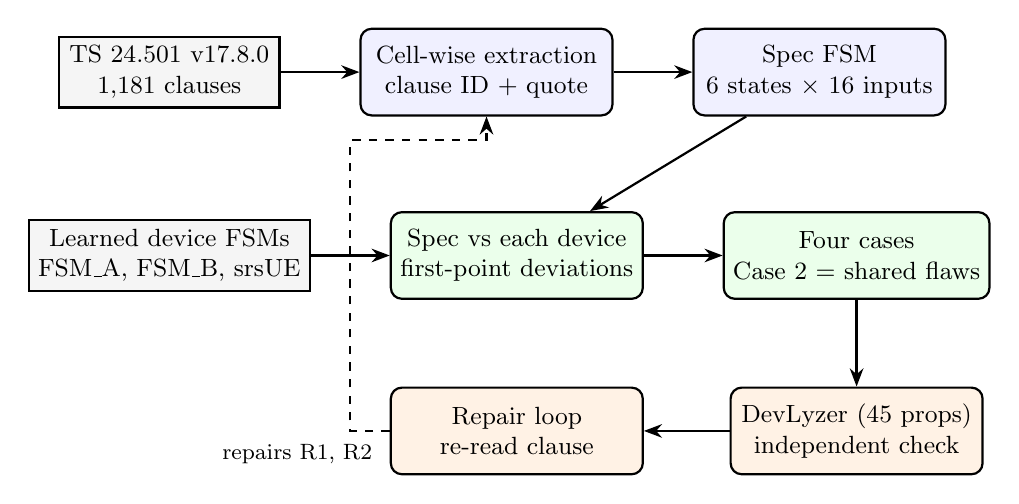
\begin{tikzpicture}[
  box/.style={draw, rounded corners, thick, minimum width=3.2cm, minimum height=1.1cm, align=center, font=\small},
  data/.style={draw, thick, minimum width=2.8cm, minimum height=0.9cm, align=center, font=\small, fill=gray!8},
  >={Stealth[length=2.3mm]}, node distance=0.9cm and 1.0cm
]
\node[data] (spec) {TS 24.501 v17.8.0\\1,181 clauses};
\node[box, fill=blue!6, right=of spec] (ext) {Cell-wise extraction\\clause ID + quote};
\node[box, fill=blue!6, right=of ext] (sfsm) {Spec FSM\\6 states $\times$ 16 inputs};
\node[data, below=1.4cm of spec] (dev) {Learned device FSMs\\FSM\_A, FSM\_B, srsUE};
\node[box, fill=green!8, right=of dev] (cmp) {Spec vs each device\\first-point deviations};
\node[box, fill=green!8, right=of cmp] (cls) {Four cases\\Case 2 = shared flaws};
\node[box, fill=orange!10, below=1.1cm of cls] (dl) {DevLyzer (45 props)\\independent check};
\node[box, fill=orange!10, below=1.1cm of cmp] (rep) {Repair loop\\re-read clause};
\draw[->, thick] (spec) -- (ext);
\draw[->, thick] (ext) -- (sfsm);
\draw[->, thick] (sfsm) -- (cmp);
\draw[->, thick] (dev) -- (cmp);
\draw[->, thick] (cmp) -- (cls);
\draw[->, thick] (cls) -- (dl);
\draw[->, thick] (dl) -- (rep);
\coordinate (gap) at ($(dev.east)!0.5!(cmp.west)$);
\draw[->, thick, dashed] (rep.west) -| ([yshift=-3mm]gap |- ext.south) -| (ext.south);
\node[font=\footnotesize, below left=0.05cm and 0.1cm of rep.west] {repairs R1, R2};
\end{tikzpicture}
\caption{Thrust 1 pipeline. Blue: specification side. Green: comparison. Orange: verification and repair.}
\end{figure}

% ---------------------------------------------------------------------------
\section{Method}

\subsection{Closed symbol vocabulary}

The learned FSMs speak the learner's symbols (e.g.\ \sym{nas_sm_cmd_ns_plain_text}), not message names.
Before any comparison I confirmed, from the modified Open5GS core source, what each of the 16 NAS input
symbols actually sends (message, security header type, MAC, ciphering, replay). Two examples that matter:
\sym{nas_sm_cmd_ns} and \sym{nas_sm_cmd_ns_plain_text} are both SECURITY MODE COMMANDs selecting 5G-IA0 with
header type 3; only the first carries a MAC. \sym{registration_accept_h4_plain_text} keeps header type 4 but
has no MAC and no ciphering, so ``plain\_text'' does not always mean header type 0. The core also asks for
SUCI in IDENTITY REQUEST, which decides which clause applies.

\subsection{Specification FSM: cell-wise, closed-world extraction}

Instead of letting an LLM invent states and transitions, I fixed six states defined in TS~24.501 terms and
filled every (state, input) cell:

\begin{table}[H]
\centering
\small
\begin{tabularx}{\textwidth}{l X}
\toprule
S0 & Before \sym{enable_s1}: UE in 5GMM-DEREGISTERED, no NAS signalling connection. \\
S1 & 5GMM-REGISTERED-INITIATED, REGISTRATION REQUEST sent, no 5G NAS security context, not authenticated. \\
S2 & 5G AKA completed (new K\textsubscript{AMF}); secure exchange of NAS messages not yet established. \\
S3 & SECURITY MODE COMMAND accepted; secure exchange established; not yet registered. \\
S4 & 5GMM-REGISTERED (REGISTRATION ACCEPT processed); secure exchange established. \\
S5 & 5GMM-DEREGISTERED after network-initiated de-registration; connection released. \\
\bottomrule
\end{tabularx}
\caption{States of the specification FSM.}
\end{table}

Each cell records the output, the next state, extra outputs a compliant UE may send (``may'' behaviour), a
\emph{kind}, the clause ID and a verbatim quote:

\begin{table}[H]
\centering
\small
\begin{tabular}{l r p{9.6cm}}
\toprule
Kind & Cells & Meaning \\
\midrule
SPEC & 53 & The quoted clause states the behaviour directly (``shall''). \\
INFERRED & 8 & Follows from the quoted clause(s), not stated for exactly this case; the gap is noted. \\
UNDERSPECIFIED & 5 & The spec does not say what the UE does; reported as (c) candidates, never as deviations. \\
NO\_CONNECTION & 30 & S0/S5: nothing can be received. \\
\midrule
Total & 96 & \textbf{89 evidence quotes, all matched after normalization} by an automatic check. \\
\bottomrule
\end{tabular}
\caption{Spec FSM cells. Clauses cited: 4.4.3.2, 4.4.4.2, 5.4.1.3.3, 5.4.2.2, 5.4.2.3, 5.4.2.5, 5.4.3.3,
5.4.4.2, 5.4.4.3, 5.5.1.2.2, 5.5.1.2.4, 5.5.1.2.7, 5.5.2.3.2, 7.4.}
\end{table}

Example cell (S3, \sym{id_request_plain_text}): output \sym{null_action}, kind SPEC, clause 4.4.4.2:
\begin{lstlisting}
"If any NAS signalling message is received as not integrity protected even though the secure
 exchange of NAS messages has been established by the network, then the NAS shall discard this
 message."
\end{lstlisting}

\subsection{Modelling the test harness}

The 5GBaseChecker core and learner answer \sym{null_action} themselves when a precondition fails (e.g.\ no
K\textsubscript{AMF} yet, no stored SMC to replay, a counter cut-off in the learner), without the UE ever
seeing a message. Every learned FSM contains these edges. I first modelled them exactly from the source
code; the learned devices immediately contradicted two of my assumptions (both devices answer an IDENTITY
REQUEST before authentication, and a protected SMC right after authentication). The final comparator
therefore treats these preconditions as \emph{uncertain}: where the harness may block a message,
\sym{null_action} is also accepted and the device's answer tells which branch happened. Only ``no
connection'' (S0, S5) is treated as certain.

\subsection{Comparison and the four cases}

For each device, the comparator walks the specification and the device FSM together over the 16 NAS inputs
and records the \emph{first} step where the device's output is not allowed by the spec (no cascades). Each
violated spec cell becomes a deviation class with its shortest witness, which is replayed on every device:

\begin{table}[H]
\centering
\small
\begin{tabular}{c l l}
\toprule
Case & Devices vs spec & Meaning \\
\midrule
1 & all conform & nothing to report \\
2 & none eligible conform, final outputs agree & invisible only if complete witness outputs agree \\
3 & some conform & devices split (DevScan can see it) \\
4 & none conform, devices disagree & each device wrong in its own way \\
\bottomrule
\end{tabular}
\caption{Four-case classification.}
\end{table}

A class is \emph{visible to differential testing} if the devices' outputs differ anywhere along its witness.
Case labels use only devices whose preceding outputs were allowed; Case~2 alone does not imply invisibility.
There are eight visible Case~2 classes as well as six invisible ones.

% ---------------------------------------------------------------------------
\section{Results}

\subsection{D2: the blind spot exists in the authors' own data}

DevScan on FSM\_A vs FSM\_B (the authors' tool, reproduced exactly: same 8 traces as shipped) reports
\textbf{8 deviations. Every one ends at} \sym{nas_sm_cmd_ns}. None ends at a plain IDENTITY REQUEST, a plain
AUTHENTICATION REQUEST, a replayed SMC or a header-type-2 SMC after security, because both devices behave
the same way there.

\subsection{D3: the specification reference closes it}

\begin{table}[H]
\centering
\small
\begin{tabular}{l r}
\toprule
First-point deviations, FSM\_A / FSM\_B & 42 / 167 \\
Deviation classes (one per violated spec cell) & 23 \\
\quad Case 2, \textbf{invisible to differential testing} & \textbf{6} \\
\quad Case 2, visible (devices differ earlier on the witness) & 8 \\
\quad Case 3 & 9 \\
DevLyzer verdict on all 23 classes & 23 property violations, 0 unresolved \\
\bottomrule
\end{tabular}
\caption{Spec vs FSM\_A and FSM\_B.}
\end{table}

\begin{table}[H]
\centering
\small
\begin{tabularx}{\textwidth}{>{\raggedright}p{3.6cm} >{\raggedright}p{3.0cm} >{\raggedright}p{1.9cm} >{\raggedright}p{1.9cm} c >{\raggedright\arraybackslash}X}
\toprule
Spec cell & Spec says (clause) & FSM\_A & FSM\_B & Issue & DevLyzer \\
\midrule
\sym{id_request_plain_text} after SMC (S3) & discard (4.4.4.2) & \sym{id_response} & \sym{id_response} & I3 & prop.\ 4 \\
\sym{auth_request_plain_text} after SMC (S3) & discard (4.4.4.2) & \sym{auth_response} & \sym{auth_response} & I4 & prop.\ 6 \\
\sym{nas_sm_cmd_replay} after SMC (S3) & discard (4.4.3.2) & \sym{nas_sm_complete} & \sym{nas_sm_complete} & I6 & props.\ 8, 9 \\
\sym{nas_sm_cmd_ns_plain_text} (S2, S3) & SECURITY MODE REJECT (5.4.2.3, 5.4.2.5) & \sym{nas_sm_complete} & \sym{nas_sm_complete} & I10 & props.\ 12, 13 \\
\sym{nas_sm_cmd_ns_plain_text} before auth (S1) & reject (inferred) & \sym{nas_sm_complete} & \sym{nas_sm_complete} & I10 & props.\ 12, 13 \\
\bottomrule
\end{tabularx}
\caption{The six Case 2 classes invisible to device-vs-device comparison (I10 appears in three states).
Both devices give the same wrong answer; the spec reference flags it with clause evidence, and the authors'
properties independently agree.}
\end{table}

\paragraph{(c) candidates: where the specification is silent.}

\begin{table}[H]
\centering
\small
\begin{tabularx}{\textwidth}{>{\raggedright}p{5cm} >{\raggedright}p{2.4cm} >{\raggedright}p{2.6cm} X}
\toprule
Cell & FSM\_A & FSM\_B & Note \\
\midrule
\sym{nas_sm_cmd_protected} (header type 2 SMC) after SMC & \sym{nas_sm_complete} & \sym{nas_sm_complete} &
  I19, paper class U1. 5.4.2.2 obliges the AMF to send SMC unciphered; the UE side is unspecified. Shared, so
  also invisible to differential testing. \\
\sym{config_update_cmd_protected} (NITZ only, no ack requested) & \sym{null_action} & \sym{config_update_complete} &
  I20, paper class U2. 5.4.4.3 says when to send COMPLETE, not that the UE must not send it otherwise. \\
\bottomrule
\end{tabularx}
\caption{Device behaviour in UNDERSPECIFIED cells. Both match the paper's ``underspecified'' classification.}
\end{table}

\subsection{Independent confirmation}

I converted all 23 deviation classes to DevLyzer's own input format (\sym{deviant-queries.json}) and ran the
unmodified DevLyzer. It classifies all 23 as property violations, 0 unresolved, and each invisible Case 2 maps
to the property one would expect (table above). The properties were written externally by the
5GBaseChecker authors. The repaired spec model uses device/property evidence, so this is not a
fully independent semantic validation. A violation can concern a witness prefix: class~23
violates property~11 through an earlier null-integrity SMC rejection, rather than its final
protected Registration Accept.

\subsection{The loop: evidence repaired the specification model}

\begin{table}[H]
\centering
\small
\begin{tabularx}{\textwidth}{l >{\raggedright}p{3.4cm} >{\raggedright}p{3.4cm} X}
\toprule
ID & Draft cell & Evidence & Clause re-read $\rightarrow$ repair \\
\midrule
R1 & S3 $\times$ protected DEREGISTRATION REQUEST $\rightarrow$ accept & DevLyzer property 1 disagreed &
  5.5.1.2.7: ``If the UE receives a DEREGISTRATION REQUEST message from the network in state
  5GMM-REGISTERED-INITIATED the de-registration procedure shall be aborted and the initial registration
  procedure shall be progressed.'' $\rightarrow$ ignore \\
R2 & S4 $\times$ second REGISTRATION ACCEPT $\rightarrow$ REGISTRATION COMPLETE & devices ignore it &
  7.4: a message not compatible with the protocol state gets 5GMM STATUS \#98, which is outside the learner's
  output alphabet $\rightarrow$ \sym{null_action} \\
\bottomrule
\end{tabularx}
\caption{Repairs of the specification model (log: \sym{spec_fsm/REPAIRS.md}).}
\end{table}

\subsection{Further findings}

\begin{itemize}[itemsep=3pt]
  \item \textbf{A gap in TS~24.501 v17.8.0.} The UE rule ``return a REGISTRATION COMPLETE message to the AMF
        to acknowledge the received 5G-GUTI'' appears only in 5.5.1.3.4 (mobility and periodic registration).
        For initial registration (5.5.1.2.4) the AMF starts T3550 and waits for REGISTRATION COMPLETE, but no
        matching UE obligation is stated. I checked the raw document: the sentence occurs exactly once.
  \item \textbf{One of the 45 expert properties is imprecise.} Property~1 uses ``never
        \sym{registration_complete}'' only in the future direction, so a UE that registered, re-keyed with a
        new SMC and is then de-registered is treated as unregistered. The properties are strong evidence, not
        ground truth.
  \item \textbf{SPEC5G cannot serve as the retrieval corpus.} I mapped SPEC5G's copy of TS~24.501 back to
        clause IDs (62\% exact matches, so it is v17.8.0 or very close), but it holds only 3,736 lines, half of
        them the change-history table; about 109 lines fall in the eight procedures Thrust~1 needs (0 in the
        identification procedure). The proposal now retrieves from the 3GPP clause index, with SPEC5G as a
        secondary source.
\end{itemize}

% ---------------------------------------------------------------------------
\section{Reproducing 5GBaseChecker (supporting work)}

\begin{table}[H]
\centering
\small
\begin{tabularx}{\textwidth}{>{\raggedright}p{4.2cm} >{\raggedright\arraybackslash}X}
\toprule
Step & Result \\
\midrule
DevScan on FSM\_A vs FSM\_B & 8 deviation traces in 5~s, \textbf{identical} to the shipped set \\
DevLyzer, 45 properties & 8/8 analysed, 0 unresolved, 2~s \\
NAS-only properties & 21 of 45 mention no RRC symbol (1--15, 29--32, 43, 44) \\
Live stack (modified Open5GS 2.4.9, srsRAN gNB 22.04.1, srsUE \sym{release_22_10}) & built and running
  over ZeroMQ in an Ubuntu 20.04 container; manual probe shows srsUE accepting a replayed SMC (I7) and a plain
  IDENTITY REQUEST after security (I3), as in the paper's Table~8 \\
srsUE learning (Table 4 configuration, 30 shipped counterexamples) & \textbf{budget-limited}: 6 states, 21 non-self-loop transitions; Table~8 recall 7/7 \\
\bottomrule
\end{tabularx}
\caption{Reproduction status.}
\end{table}

Problems found and fixed while bringing the live stack up (details in the progress log): the shipped learner
jar has no main class in its manifest; the gNB's learner port lacks \sym{SO_REUSEADDR}; srsUE~22.10 searches
the SSB on a different frequency than this gNB transmits; with the core's ciphering setting (NEA2 first)
srsUE fails to decode every ciphered NAS message, so srsUE runs with NEA0 (cause not yet known); the shipped
\sym{CE_reverse_feeding/srsue.properties} names \sym{device = oai}; and in counterexample-feeding mode the
learner stops after 30 equivalence queries, so exact Table~4 reproduction is not established: this hypothesis matches the six-state count
but has 21 rather than 20 transitions, and its query counts are not directly comparable.

% ---------------------------------------------------------------------------
\section{Finalized srsUE Experiment}
The analyzed artifact is \sym{hypothesis_5.dot}, preserved as
\sym{srsue_learnedModel.dot} for compatibility with the analysis scripts.
Its provenance records that it is a budget-limited hypothesis, not a converged model.
The learner's \sym{LogOracle} invokes \sym{System.exit(0)} after 30 equivalence-query calls
in counterexample-feeding mode, before the normal final-model writer can run.
Repeated resumes reproduced the same model hash and then exited at the same budget.

\begin{center}
\begin{tabular}{lrr}
\toprule
Metric & Paper & This experiment \\
\midrule
States & 6 & 6 \\
Non-self-loop transitions & 20 & 21 \\
Expected Table~8 NAS issues recovered & 7 & 7 \\
\bottomrule
\end{tabular}
\end{center}
Both I9 variants are present; I9 counts once in the seven-issue recall.
I6 is also present, although the paper's Table~8 lists it only for OAI UE.
The transition-count difference is retained as an experimental difference.
With FSM\_A, FSM\_B and srsUE, the comparator returns 23 classes:
6 invisible Case~2, 8 visible Case~2, and 9 visible Case~3.
DevLyzer classifies all 23 witness records as attack traces, with seven benign records and zero unresolved records.
The attack and benign sets overlap: a witness can include violating and benign device-output groups.
This is property-level corroboration, not proof of exploit impact or of every spec-cell interpretation.
Textual quote verification alone does not establish semantic correctness.

\section{Supplementary Review and Teacher-Review Milestone}
The current deliverable is the finalized demonstration for teacher feedback;
the full research plan remains open. The user will compile this source in Overleaf.
A clause-based review of 30 selected cells is saved in
\sym{results/T1_SEMANTIC_REVIEW.json}. It saw the existing model and is not a
blind extraction ensemble or an independent human reference evaluation.
Sensitivity testing retains six invisible witnesses after either correcting
optional SMC next-state handling or allowing R2's disputed COMPLETE alternative.
Suppressing judgments on INFERRED cells leaves five invisible witnesses.

Supplemental D4 experiments used actual LearnLib TTT and Wp (lookahead 1, 29
inputs) against fixed saved FSM oracles. Exact equivalence checks passed in all
12 runs. SPEC guidance reduced EQ calls by 5.65--12.47\% versus Wp alone;
shipped guidance performed better. These results do not measure live UE query
savings or radio runtime. See \sym{results/D4_OFFLINE.md} for counts.
The isolated live baseline was stopped for this review milestone and its partial
logs preserved. OAI reproduction, live D4 and independent extraction/reference
validation are deferred until teacher feedback. The original budget-limited
srsUE model and main comparison remain unchanged.

\section{Limitations}

\begin{itemize}[itemsep=3pt]
  \item \textbf{Extraction.} The spec FSM was extracted by Claude inside a Claude Code session (no API key
        available), one sample per cell, no ensemble vote. All 89 evidence quotes are checked for textual presence, but a scripted, repeated
        extraction with an API model is needed before publication.
  \item \textbf{Ground truth for FSM\_A/FSM\_B.} Their device identities are not published, so their ground
        evidence here is DevLyzer property verdicts, rather than device-specific Table~8 truth. Table~8 applies to srsUE (7/7 recovered here) and OAI UE (not run here).
  \item \textbf{Harness.} Where the core or learner may suppress a message, \sym{null_action} is always
        accepted, so a device that wrongly stays silent in exactly those situations is not flagged. Findings
        where a device answers when it must not (I3, I4, I6, I10) are unaffected.
  \item \textbf{Coverage of S4.} FSM\_A never completes registration (it ignores REGISTRATION ACCEPT, issue
        I17), so the two-device registered-state results rely on FSM\_B; the three-device analysis also includes srsUE.
  \item \textbf{Novelty claim.} The issues found are known issues; recovering them is the validation of the
        method. The contribution claimed is the method and its measured effect on the blind spot.
\end{itemize}

% ---------------------------------------------------------------------------
\section{Next Steps}

\begin{enumerate}[itemsep=3pt]
  \item Remove the learner's hard-coded query-budget exit and perform a separate convergence run if a
        converged model is required. The finalized result here is hypothesis 5.
  \item Re-run the extraction as a script (several samples per cell, majority vote) and measure agreement with
        this version and PSMBench F1 against a hand-built reference for SMC and registration.
  \item Guided learning (D4): turn spec transitions into potential counterexamples for the learner and measure
        the saving in equivalence queries against the Wp-method alone.
  \item Optional: OAI UE over the RF simulator, for the exact two-UE setup of the paper.
\end{enumerate}

% ---------------------------------------------------------------------------
\section*{References}
\small
[1] K.~Tu, A.~Al~Ishtiaq, S.~M.~M.~Rashid, Y.~Dong, W.~Wang, T.~Wu, S.~R.~Hussain. Logic Gone Astray: A Security
Analysis Framework for the Control Plane Protocols of 5G Basebands. USENIX Security 2024.\\
{[2]} Z.~Shen, X.~Luo, I.~Karim, E.~Bertino. PSMBench: A Benchmark and Dataset for Evaluating LLMs Extraction of
Protocol State Machines from RFC Specifications. NeurIPS D\&B 2025.\\
{[3]} I.~Karim et al. SPEC5G: A Dataset for 5G Cellular Network Protocol Analysis. IJCNLP-AACL 2023.\\
{[4]} 3GPP TS 24.501 v17.8.0. Non-Access-Stratum (NAS) protocol for 5G System (5GS); Stage 3. 2022-09.

\normalsize
% ---------------------------------------------------------------------------
\appendix
\section{Artifacts}

All in the repository under \sym{thrust1/}:
\begin{itemize}[itemsep=1pt]
  \item \sym{symbols/alignment.md}, \sym{symbols/fsm_tools.py} --- symbol table; FSM statistics, NAS projection,
        issue probes, NuSMV property check
  \item \sym{extract/spec_clauses.py} --- TS~24.501 Word file to clause index
  \item \sym{extract/author_spec_cells.py}, \sym{spec_fsm/spec_cells_v1.json} --- the 96 spec cells with quotes
  \item \sym{extract/build_spec_fsm.py} --- quote check, PSMBench JSON, spec $\otimes$ harness FSM
  \item \sym{compare/spec_vs_devices.py} --- deviations, four cases, (c) candidates
  \item \sym{results/T1_RESULTS_v1.md}, \sym{results/T1.6_spec_vs_AB.json} --- results
  \item \sym{spec_fsm/REPAIRS.md} --- repair log; \sym{T1_PROGRESS.md} --- full engineering log
  \item \sym{env/} --- Dockerfiles, launch scripts and configs for the learning stack
\end{itemize}

\end{document}
